%%%%%%%%%%%%%%%%%%%%%%%%%%%%%%%%%%%%%%%%%%%%%%%%%%%%%%%%%%%%%%%%%%%%%%
% How to use writeLaTeX: 
%
% You edit the source code here on the left, and the preview on the
% right shows you the result within a few seconds.
%
% Bookmark this page and share the URL with your co-authors. They can
% edit at the same time!
%
% You can upload figures, bibliographies, custom classes and
% styles using the files menu.
%
%%%%%%%%%%%%%%%%%%%%%%%%%%%%%%%%%%%%%%%%%%%%%%%%%%%%%%%%%%%%%%%%%%%%%%

\documentclass[12pt]{article}

\usepackage{sbc-template}

\usepackage{graphicx,url}

%\usepackage[brazil]{babel}   
\usepackage[utf8]{inputenc}  

     
\sloppy

%\setlength{\parindent}{0pt}

\title{Assignment 1 - Gerador de Ciclos}
\author{Lara Brígida Rezende Souza\inst{1}, Matheus Moreira Sorrentino\inst{2} }


\address{Departamento de Ciência da Computação -- PUC-Minas\\
  Belo Horizonte, MG -- Brasil
\nextinstitute
  Departamento de Ciência da Computação -- PUC-Minas\\
  Belo Horizonte, MG -- Brasil
  \email{lara.brigida@sga.pucminas.br, matheus.sorrentino@sga.pucminas.br
  }
}

\begin{document} 

\maketitle

\begin{abstract}
  This meta-paper addresses two different ways of solving the problem of enumerating all existing cycles in a graph. One of the solutions is based on the permutation of the graph's vertices and the other is based on walking the graph, also known as Depth-First Search. The article provides a comparative analysis between the two solutions, which determine the differences in performance for solving the problem, especially as the size of the graph increases.
\end{abstract}
     
\begin{resumo} 
  Este meta-artigo aborda duas formas distintas de resolução para o problema de se enumerar todos os ciclos existentes em um grafo. Uma das soluções é baseada na permutação dos vértices do grafo e a outra é baseada em caminhamento no grafo, também conhecida como Busca em Profundidade. O artigo traz uma análise comparativa entre as duas soluções, visando determinar as diferenças nos desempenhos para a resolução do problema, principalmente na medida que o tamanho do grafo aumenta.
\end{resumo}


\section{Introdução}

Um ciclo em um grafo não-direcionado simples é um caminho fechado sem vértices repetidos. Mais precisamente, um ciclo é uma sequência $(v_0,a_1,v_1,a_2,v_2,...,a_k,v_k)$ com $k > 2$ em que $v_k = v_0$, mas $v_0,v_1,v_2,...,v_{k-1}$ são distintos dois a dois. Em grafos simples, pode-se representar um ciclo apenas pela sequência de vértices (uma vez que só pode existir uma única aresta entre cada par de vértices).
\\ \\
O problema de se enumerar todos os ciclos existentes em um grafo apresenta várias aplicações e pode ser resolvido por diferentes abordagens. Neste artigo veremos a implementação de duas formas distintas de resolução deste problema, fazendo uma análise comparativa entre elas: (i) uma baseada na permutação dos vértices do grafo; e (ii) outra baseada em caminhamento no grafo.
\\ \\
A divisão do trabalho se deu da seguinte forma: 
\begin{itemize}
    \item A aluna Lara Brígida ficou responsável pela implementação do algoritmo baseado em caminhamento no grafo e pela elaboração do relatório escrito. \\
    \item O aluno Matheus Moreira ficou responsável pela implementação do algoritmo baseado na permutação dos vértices do grafo e pela revisão do relatório escrito.
\end{itemize}

\section{Detalhes da implementação} \label{sec:firstpage}

\textbf{Nota:} Todo os arquivos de código-fonte contém comentários e documentação. Favor consultá-los para mais informações sobre o funcionamento do código.
\\ \\
No código implementado, a classe $"Graph"$ representa um grafo não direcionado usando uma lista de adjacências, onde cada vértice é representado por um índice na lista e as arestas são representadas pelos elementos nas listas correspondentes aos vértices.
\\ \\
O método $"addEdge"$ adiciona uma aresta entre dois vértices. O método $"printAllCyclesDFS"$ é responsável por iniciar a busca por ciclos em todos os vértices do grafo usando uma abordagem de busca em profundidade (DFS - Depth-First Search), este método explora recursivamente os vizinhos de cada vértice. O método $"printAllCyclesPermutation"$ é responsável por encontrar ciclos no grafo através de uma abordagem de permutação de vértices, este método gera todas as permutações possíveis dos vértices do grafo e verifica se cada permutação forma um ciclo. Na função $main()$, um único grafo $g$ é criado com 4 vértices e arestas entre eles são adicionadas, para este grafo, os dois métodos recém-adicionados, $"printAllCyclesDFS"$ e $"printAllCyclesPermutation"$, são chamados separadamente.
\\ \\
Para cada método de busca de ciclo, o tempo de execução é medido usando a biblioteca $"chrono"$ e, no final, os ciclos encontrados por cada método e o tempo de execução correspondente são impressos na saída padrão.

\section{Experimentos e resultados}

Nesta seção iremos discutir a respeito dos experimentos realizados para a resolução do problema e quais são os resultados gerados.

\subsection{Experimentos}

Para realizar os testes e ter uma melhor análise da eficiência de cada algorimto foram criados três tipos de grafos, um menor, um moderado e um maior. Para cada um desses grafos foi realizada cada uma das buscas, uma baseada em permutação e a outra em caminhamento, ou em profundidade.

\subsection{Resultados}

 Apesar do algoritmo baseado em permutação ser menos eficiente que o de caminhamento, para grafos menores ainda é utilizável. Contudo, a abordagem de permutação pode se tornar extremamente ineficiente para grafos de tamanho moderado ou grande, enquanto a abordagem de busca em profundidade é muito mais eficiente e prática na maioria dos casos. \\ \\ Os testes foram efetuados em um computador com a seguinte configuração:

\textbf{Sistema operacional:} Microsoft Windows 11

\textbf{Versão do sistema operacional:} 10.0.22631

\textbf{CPU:} Intel64 Family 6 Model 140 Stepping 1 GenuineIntel @ 2,803 Ghz

\textbf{Versão do GCC/G++:} 13.2.0

\begin{table}[ht]
    \begin{tabular}{|c|c|c|}
    \hline
    ~                           & Algoritmo de permutação          & DFS                      \\
    Complexidade                & O(V!)                   & O(V + E)                 \\
    \hline
    Tempo de execução - Grafo 1 & 5,926 segundos  & 4,515 segundos segundos\\
    \hline
    Tempo de execução - Grafo 2 & 1,059 segundos  & 4,792 segundos\\
    \hline
    Tempo de execução - Grafo 3 & 8,5137 x $10^{4}$ segundos  & 1,1426 x $10^{2}$ segundos\\ 
    \hline    
    \end{tabular}
\end{table} 

\begin{figure}[htbp]
  \centering
  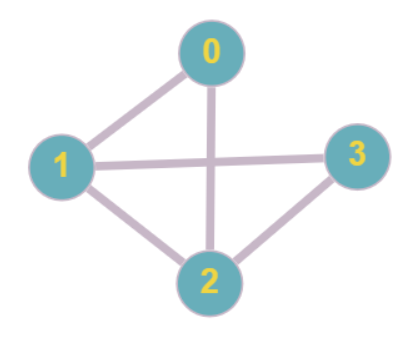
\includegraphics[width=0.5\textwidth]{grafo_01.png}
  \caption{Grafo 01}
  \label{fig:sua-imagem}
\end{figure}

\begin{figure}[htbp]
  \centering
  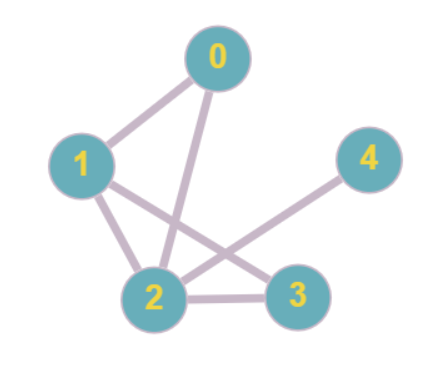
\includegraphics[width=0.5\textwidth]{grafo_02.png}
  \caption{Grafo 02}
  \label{fig:sua-imagem}
\end{figure}

\begin{figure}[htbp]
  \centering
  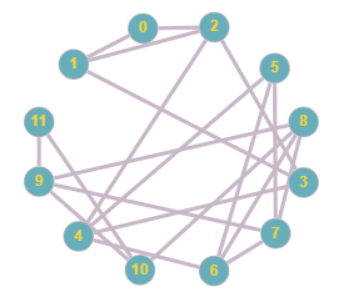
\includegraphics[width=0.5\textwidth]{grafo_03.png}
  \caption{Grafo 03}
  \label{fig:sua-imagem}
\end{figure}

\section{Conclusões}

Pode-se observar, através da tabela, que o algoritmo com base em caminhamento no grafo, algoritmo de Busca em Profundidade, teve um tempo de execução melhor que o algoritmo baseado na permutação dos vértices do grafo no primeiro e no terceiro grafos. Contudo, ambos podem ser utilizados para a detecção de ciclos em grafos conexos não-direcionados, porém, quando a performance é levada em conta, a melhor alternativa seria o algoritmo baseado em caminhamento no grafo, ainda mais em grafos de tamanho maior.

\bibliography{sbc-template}

\end{document}
